\newpage
\section{Результаты измерений}

\begin{table}[!ht]
    \centering
    \caption{Линия натрия}
    \begin{tabular}{|l|l|}
\hline
$n$ & $x,\;\text{мм}$\\\hline
$1$ & $146{,}7700 \pm 0{,}0010$\\\hline
$2$ & $147{,}7700 \pm 0{,}0010$\\\hline
$3$ & $148{,}5500 \pm 0{,}0010$\\\hline
$4$ & $148{,}8800 \pm 0{,}0010$\\\hline
$5$ & $149{,}5500 \pm 0{,}0010$\\\hline
$6$ & $150{,}5430 \pm 0{,}0010$\\\hline
$7$ & $151{,}7320 \pm 0{,}0010$\\\hline
$8$ & $152{,}8650 \pm 0{,}0010$\\\hline
$9$ & $154{,}4560 \pm 0{,}0010$\\\hline
$10$ & $156{,}4330 \pm 0{,}0010$\\\hline
$11$ & $162{,}4330 \pm 0{,}0010$\\\hline
$12$ & $164{,}2130 \pm 0{,}0010$\\\hline
$13$ & $165{,}7810 \pm 0{,}0010$\\\hline
$14$ & $166{,}9760 \pm 0{,}0010$\\\hline
$15$ & $167{,}9900 \pm 0{,}0010$\\\hline
$16$ & $168{,}8470 \pm 0{,}0010$\\\hline
$17$ & $169{,}7920 \pm 0{,}0010$\\\hline
$18$ & $170{,}5420 \pm 0{,}0010$\\\hline
$19$ & $171{,}2750 \pm 0{,}0010$\\\hline
$20$ & $171{,}8610 \pm 0{,}0010$\\\hline
\end{tabular}

\end{table}

\begin{table}[!ht]
    \centering
    \caption{Зеленая линия ртути}
    \begin{tabular}{|l|l|}
\hline
$n$ & $x,\;\text{мм}$\\\hline
$1$ & $153{,}5750 \pm 0{,}0010$\\\hline
$2$ & $155{,}8780 \pm 0{,}0010$\\\hline
$3$ & $158{,}0080 \pm 0{,}0010$\\\hline
$4$ & $161{,}1760 \pm 0{,}0010$\\\hline
$5$ & $164{,}6600 \pm 0{,}0010$\\\hline
$6$ & $176{,}8020 \pm 0{,}0010$\\\hline
$7$ & $181{,}5900 \pm 0{,}0010$\\\hline
$8$ & $184{,}2700 \pm 0{,}0010$\\\hline
$9$ & $186{,}6420 \pm 0{,}0010$\\\hline
$10$ & $188{,}5200 \pm 0{,}0010$\\\hline
\end{tabular}

\end{table}

\begin{table}[!ht]
    \centering
    \caption{Желтая линия ртути 1}
    \begin{tabular}{|l|l|}
\hline
$n$ & $x,\;\text{мм}$\\\hline
$1$ & $188{,}2290 \pm 0{,}0010$\\\hline
$2$ & $186{,}2000 \pm 0{,}0010$\\\hline
$3$ & $183{,}8100 \pm 0{,}0010$\\\hline
$4$ & $180{,}4800 \pm 0{,}0010$\\\hline
$5$ & $175{,}0350 \pm 0{,}0010$\\\hline
$6$ & $167{,}1850 \pm 0{,}0010$\\\hline
$7$ & $161{,}6300 \pm 0{,}0010$\\\hline
$8$ & $158{,}4040 \pm 0{,}0010$\\\hline
$9$ & $155{,}7460 \pm 0{,}0010$\\\hline
$10$ & $153{,}6300 \pm 0{,}0010$\\\hline
\end{tabular}

\end{table}

\begin{table}[!ht]
    \centering
    \caption{Желтая линия ртути 2}
    \begin{tabular}{|l|l|}
\hline
$n$ & $x,\;\text{мм}$\\\hline
$1$ & $189{,}9000 \pm 0{,}0010$\\\hline
$2$ & $188{,}0550 \pm 0{,}0010$\\\hline
$3$ & $186{,}1500 \pm 0{,}0010$\\\hline
$4$ & $183{,}5000 \pm 0{,}0010$\\\hline
$5$ & $180{,}2650 \pm 0{,}0010$\\\hline
$6$ & $174{,}4000 \pm 0{,}0010$\\\hline
$7$ & $167{,}8650 \pm 0{,}0010$\\\hline
$8$ & $161{,}8100 \pm 0{,}0010$\\\hline
$9$ & $158{,}4650 \pm 0{,}0010$\\\hline
$10$ & $156{,}0550 \pm 0{,}0010$\\\hline
$11$ & $153{,}9460 \pm 0{,}0010$\\\hline
$12$ & $151{,}6800 \pm 0{,}0010$\\\hline
\end{tabular}

\end{table}

\newpage
~
\newpage

Параметры установки с натриевой лампой: $f = 50\;\text{мм}$, $L = 90\;\text{мкм}$.

Параметры установки с ртутной лампой: $f = 110\;\text{мм}$, $L = 100\;\text{мкм}$.

Ширина линии натрия $\delta r = 449 \pm 1\;\text{мкм}$, зеленой линии ртути $2036 \pm 1\;\text{мкм}$, первой желтой линии ртути $4070 \pm 1\;\text{мкм}$, второй желтой линии ртути $2778 \pm 1\;\text{мкм}$.


\begin{figure}[ht!]
    \center{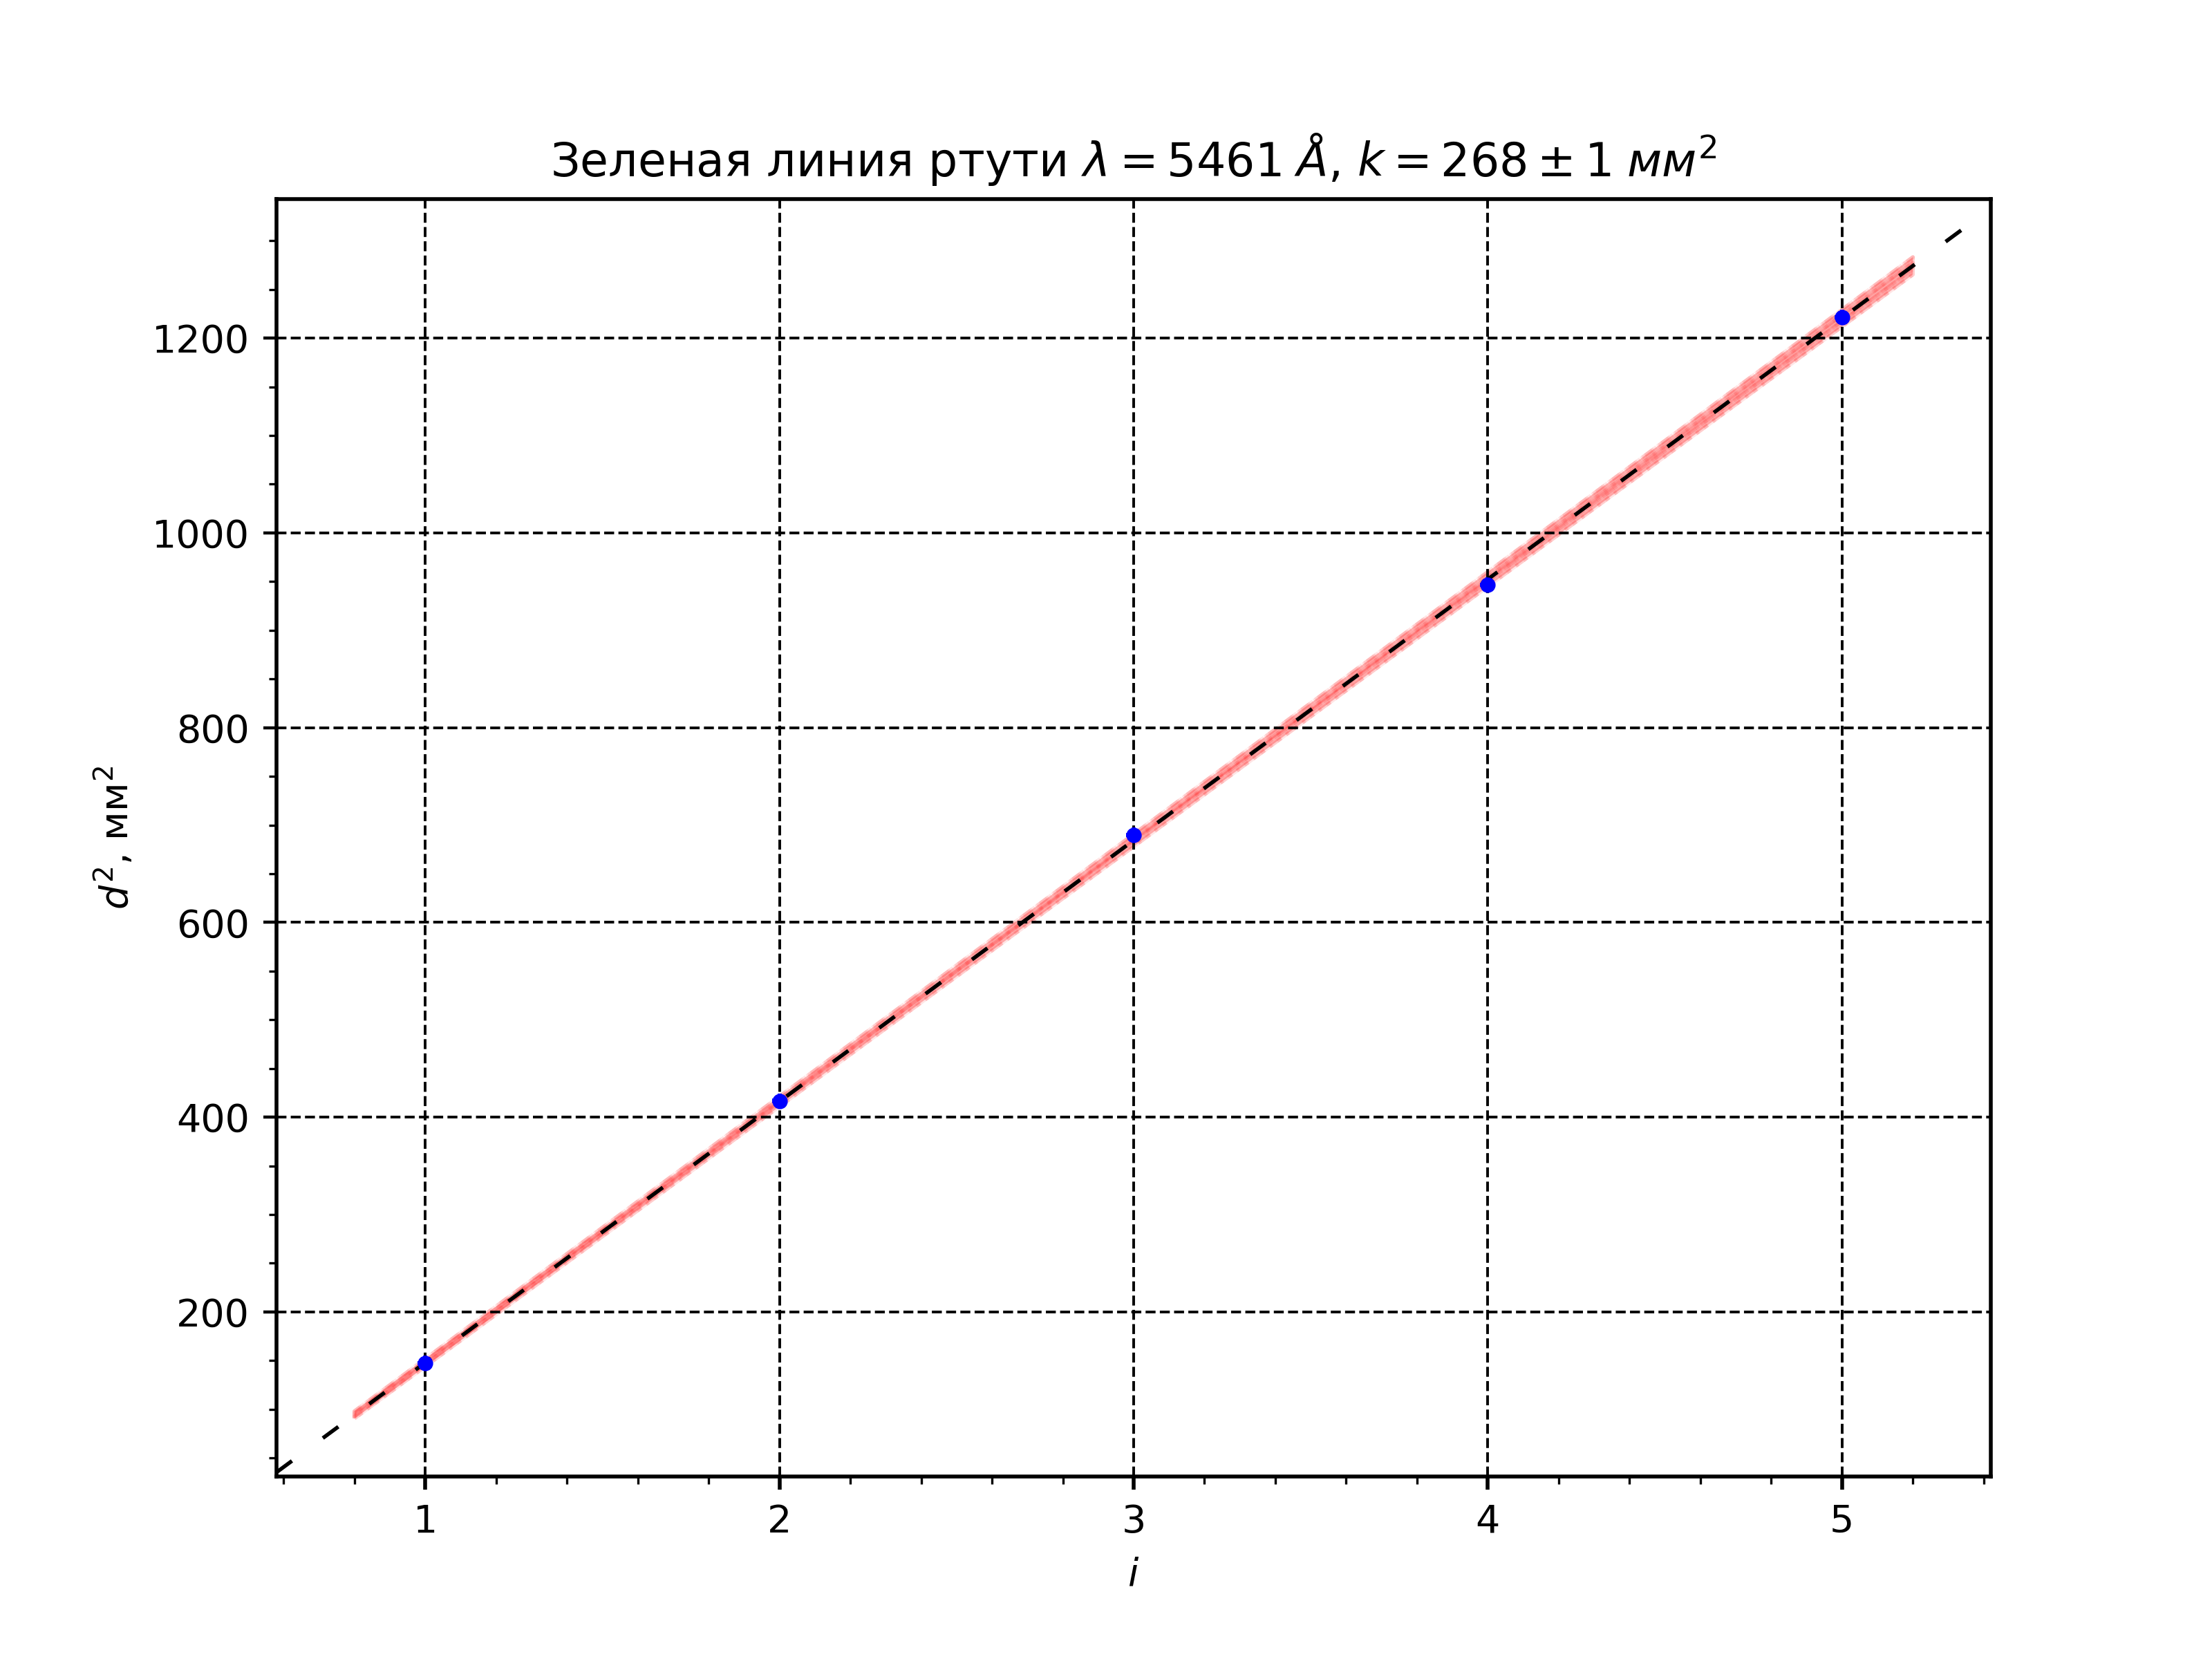
\includegraphics[width=0.8\linewidth]{../img/plothg.png}}
\end{figure}
\begin{figure}[ht!]
    \center{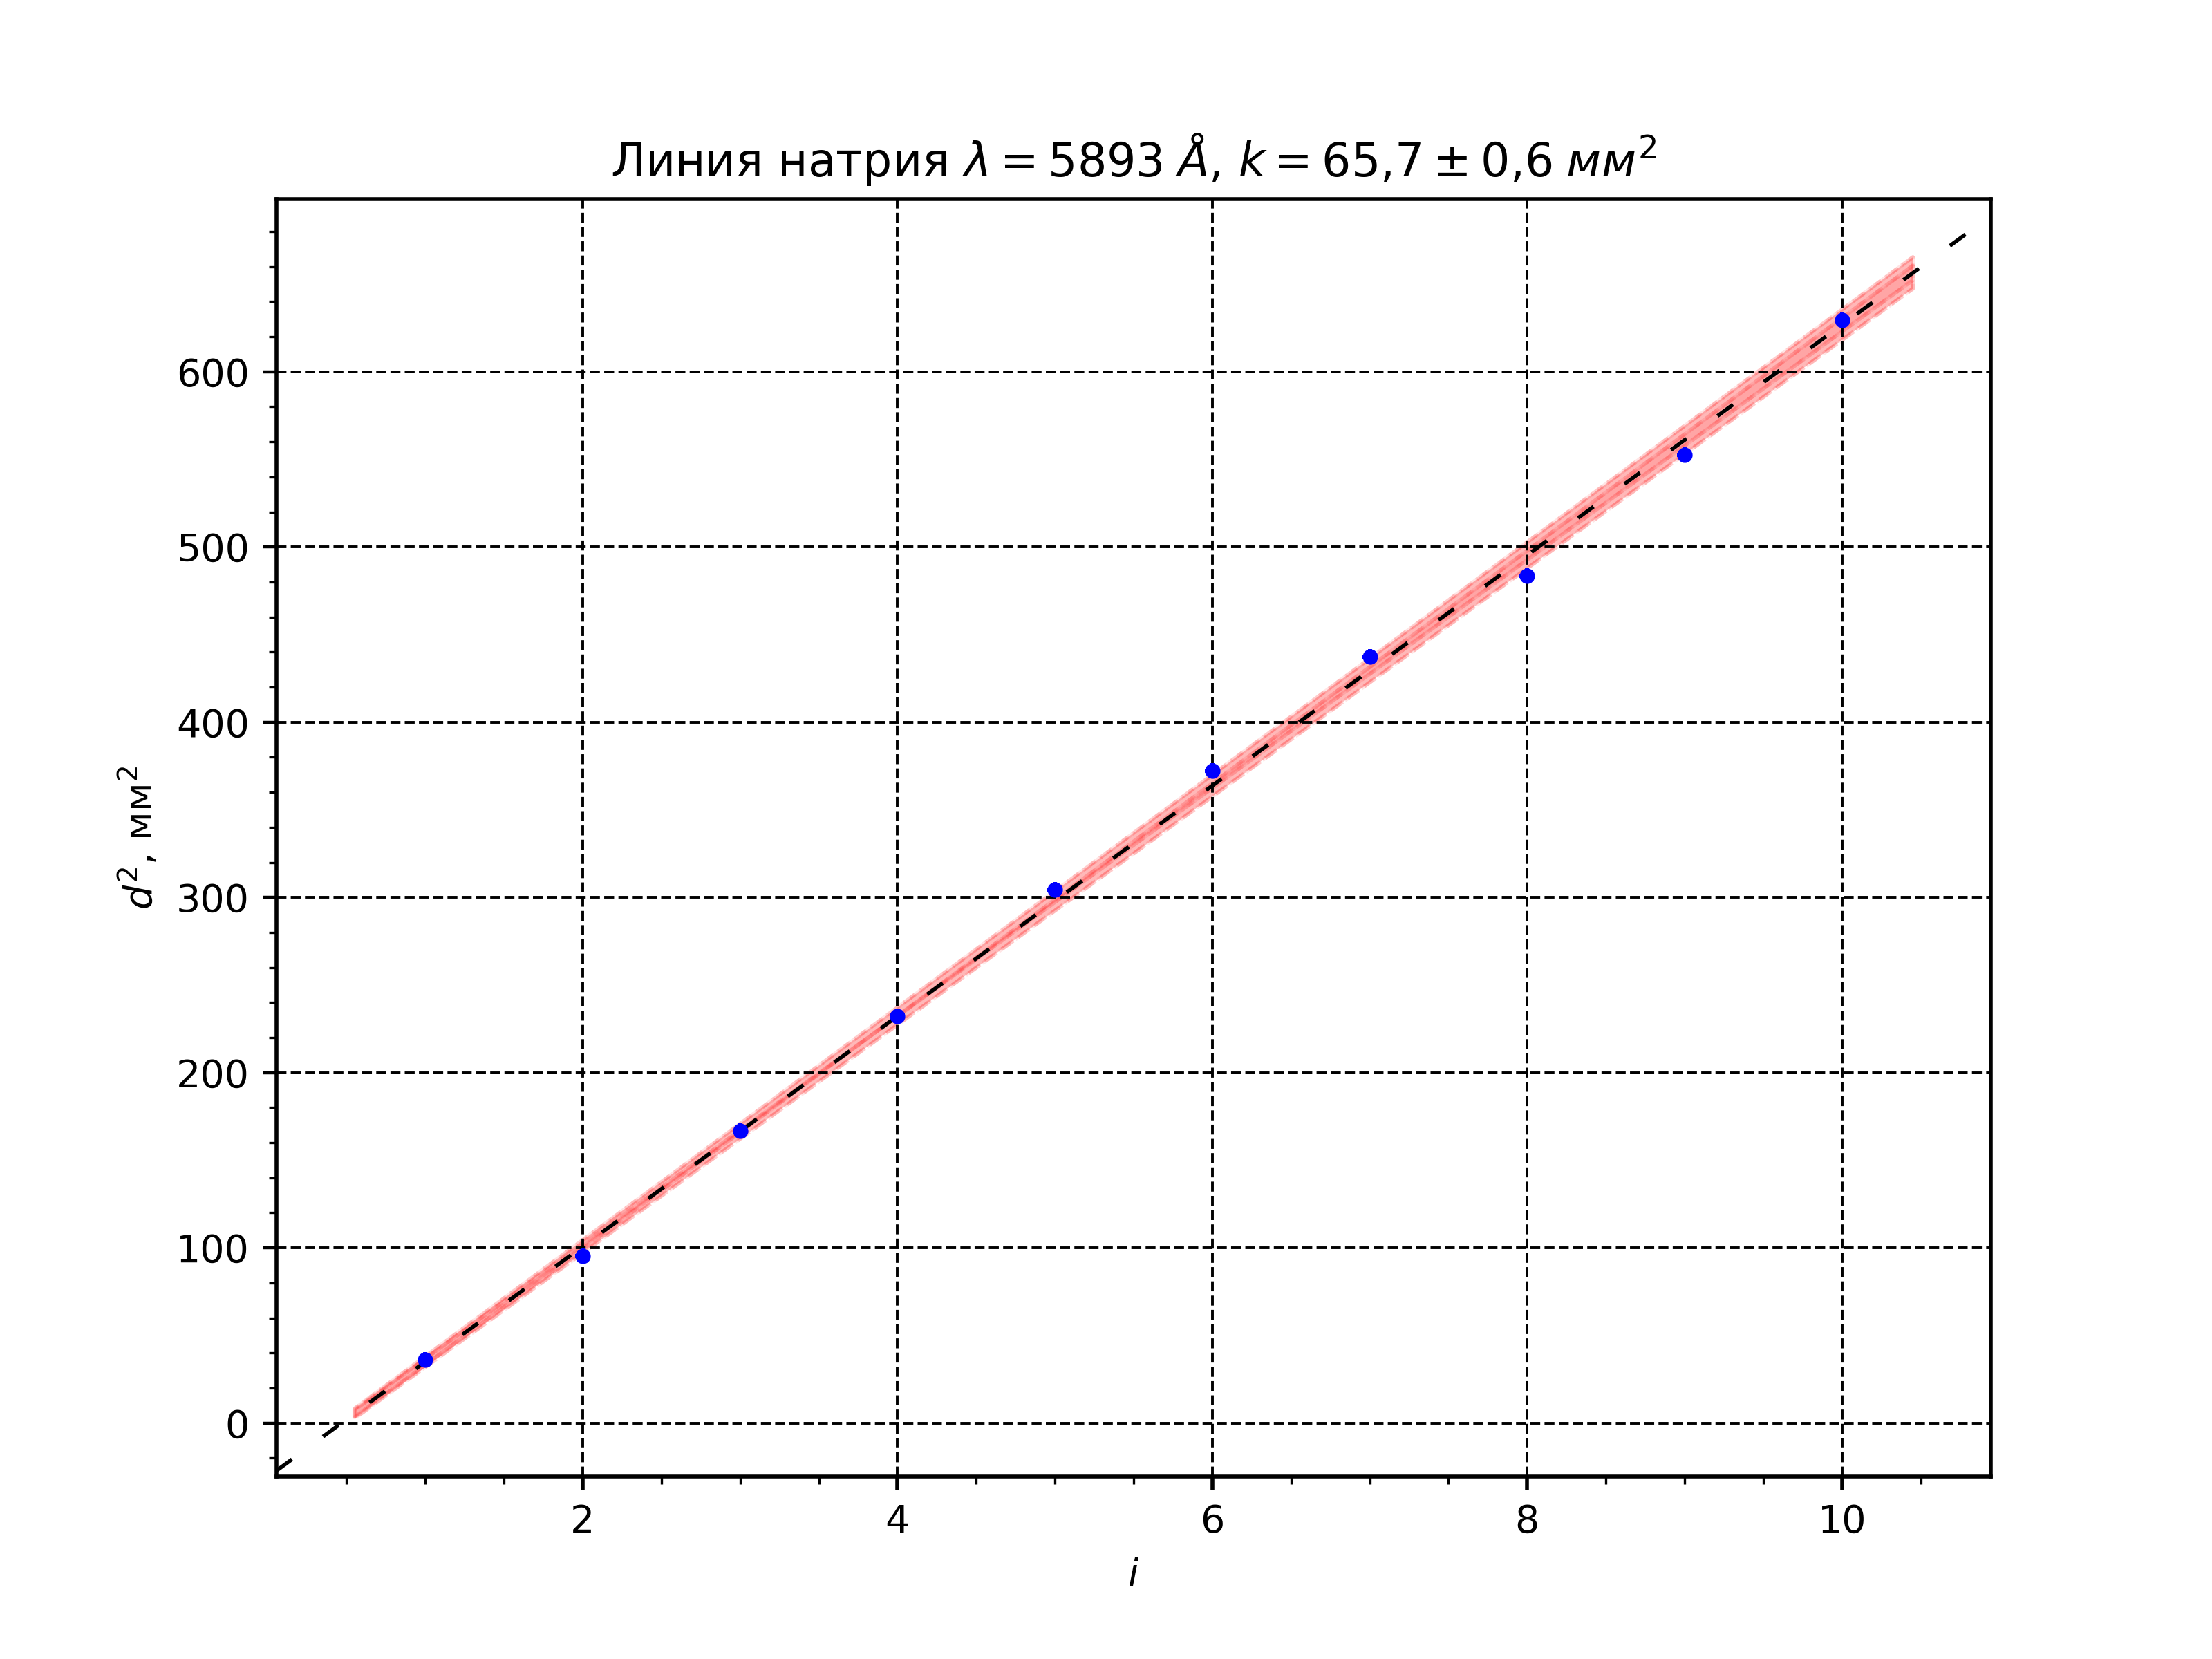
\includegraphics[width=0.8\linewidth]{../img/plotna.png}}
\end{figure}

$L = 4 \lambda f ^{ 2} / k$. $L_{\text{Na}} = 89{,}6 \pm 0{,}9\;\text{мкм}$. $L_{\text{Hg}} = 98{,}6 \pm 0{,}4 \;\text{мкм}$.

Максимальный порядок интерференции $m = 2L / \lambda \approx 350$.

Дисперсионная область $ \Delta \lambda = \lambda / m \approx 16\; \si{\angstrom}$

$R_{\text{апп}} = \frac{4f^{2}}{d\delta r}$. $R_{\text{Na}} = 3710 \pm 10$, $N_{\text{Na}} = R_{\text{Na}} / m \approx 11$. $R_{\text{Hg}} = 1958 \pm 1$, $N_{\text{Na}} \approx 6 $. 

$R_{\text{теор}} = \frac{ \pi \sqrt{r}}{1 - r} m \approx 6800$, $N_{\text{теор}} = \frac{ \pi \sqrt{r}}{1 - r} \approx 19$
